\item Per la scuola Marco acquista dei quaderni da 1,80 euro ciascuno e spende in tutto 9,00 euro. Scrivi l'operazione da fare per calcolare quanti quaderni ha acquistato Marco e scrivi il risultato.
\begin{figure}[h]
	\centering
		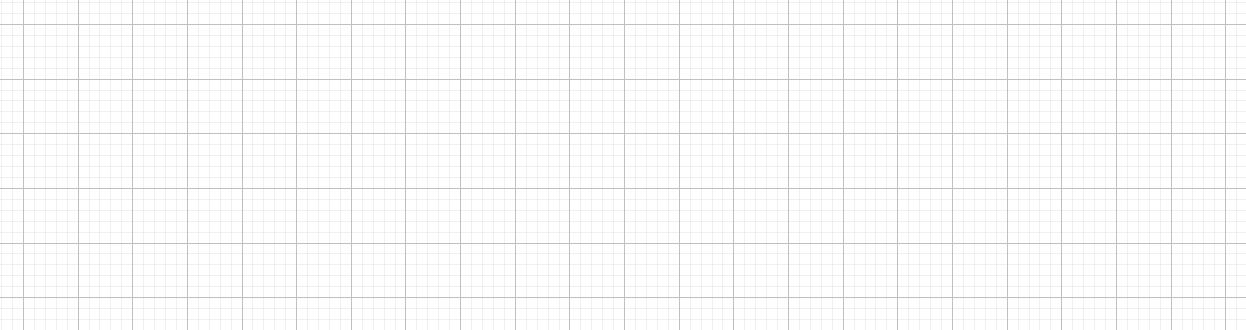
\includegraphics[width=13cm]{figure/quadretti.png}
\end{figure}
